% updated April 2002 by Antje Endemann
% Based on CVPR 07 and LNCS, with modifications by DAF, AZ and elle, 2008 and AA, 2010, and CC, 2011; TT, 2014; AAS, 2016; AAS, 2020

\documentclass[runningheads]{llncs}
\usepackage{graphicx}
\usepackage{comment}
\usepackage{amsmath,amssymb} % define this before the line numbering.
\usepackage{color}
\usepackage{wrapfig}
\usepackage{adjustbox}
\usepackage{booktabs}
\usepackage{enumitem}
\usepackage{xr}
% INITIAL SUBMISSION - The following two lines are NOT commented
% CAMERA READY - Comment OUT the following two lines
\usepackage[width=122mm,left=12mm,paperwidth=146mm,height=193mm,top=12mm,paperheight=217mm]{geometry}
\usepackage[ruled,linesnumbered]{algorithm2e}
\usepackage[colorlinks, backref=page]{hyperref}
% our math commands
\input{math_commands.tex}

\begin{document}
% \renewcommand\thelinenumber{\color[rgb]{0.2,0.5,0.8}\normalfont\sffamily\scriptsize\arabic{linenumber}\color[rgb]{0,0,0}}
% \renewcommand\makeLineNumber {\hss\thelinenumber\ \hspace{6mm} \rlap{\hskip\textwidth\ \hspace{6.5mm}\thelinenumber}}
% \linenumbers
\pagestyle{headings}
\mainmatter
\def\ECCVSubNumber{5237}  % Insert your submission number here

\title{Universal Differentiable Renderer \\for Implicit Neural Representations} % Replace with your title

% INITIAL SUBMISSION 
\begin{comment}
\titlerunning{ECCV-20 submission ID \ECCVSubNumber} 
\authorrunning{ECCV-20 submission ID \ECCVSubNumber} 
\author{Anonymous ECCV submission}
\institute{Paper ID \ECCVSubNumber}
\end{comment}
%******************

% CAMERA READY SUBMISSION
% \begin{comment}
\titlerunning{Universal Differentiable Renderer for Implicit Neural Representations}
% If the paper title is too long for the running head, you can set
% an abbreviated paper title here
%
\author{Lior Yariv \and
Matan Atzmon \and
Yaron Lipman}
%
\authorrunning{L. Yariv, M. Atzmon, Y. Lipman}
% First names are abbreviated in the running head.
% If there are more than two authors, 'et al.' is used.
%
\institute{Weizmann Institute of Science}
% \end{comment}
%******************
\maketitle

\begin{abstract}
The goal of this work is to learn implicit 3D shape representation with 2D supervision (\ie, a collection of images).  To that end we introduce the Universal Differentiable Renderer (UDR) a neural network architecture that can provably approximate reflected light from an implicit neural representation of a 3D surface, under a wide set of reflectance properties and lighting conditions. Experimenting with the task of multiview 3D reconstruction, we find our model to improve upon the baselines in the accuracy of the reconstructed 3D geometry and rendering from unseen viewing directions.

%, which can be attributed to a better separation of geometry and reflectance/lighting properties by the UDR.


%\keywords{3D }
\end{abstract}


\section{Introduction}

Learning 3D shapes with 2D supervision (\ie, images) is a fundamental computer vision problem. A recent successful neural networks approach to solve this problem is to use a differentiable rendering system coupled with a choice of 3D geometry representation. Differential rendering systems are mostly based on ray casting/tracing \cite{sitzmann2019scene,niemeyer2019differentiable,li2018differentiable,liu2019learning,saito2019pifu,liu2019dist}, or rasterization  \cite{loper2014opendr,kato2018neural,genova2018unsupervised,liu2019soft_b,chen2019learning}, while popular models to represent 3D geometry include point clouds \cite{yifan2019differentiable}, triangle meshes \cite{chen2019learning}, implicit representations defined over volumetric grids \cite{jiang2019sdfdiff}, and recently also neural implicit representations, namely, zero level sets of neural networks \cite{liu2019learning,niemeyer2019differentiable}. 

The main benefit in implicit neural representations is their flexibility to represent surfaces with arbitrary shape and topology, and produce smooth surface approximation without a fixed discretization, in contrast to, \eg, an implicit function defined over a volumetric grid or a triangle mesh. Thus far, differentiable rendering systems with implicit neural representations \cite{liu2019learning,liu2019dist,niemeyer2019differentiable} did not incorporate lighting and reflectance properties required for producing faithful appearance of 3D geometry in images. The main challenge seems to be relating, in a differentiable way properties of the implicit surface and the parameters of the neural network representing it. 

The goal of this paper is to introduce the Universal Differentiable Renderer (UDR) for implicit neural representations. That is, a differentiable renderer that is \emph{provably} able to approximate the reflected light from a 3D shape represented as a zero level set of a neural network with an arbitrary bidirectional reflectance distribution function (BRDF) and lighting conditions from a certain family. Although the BRDF/lighting family we consider in this paper is not the most general one, as it excludes secondary lighting effects, it includes, or can approximate with arbitrary precision, many real-life appearances of 3D surfaces. 

We represent the geometry as the zero level set of neural network and use the recent implicit (Eikonal) regularization \cite{gropp2020implicit} to produce an approximated signed distance function. For the UDR we require differentiable (w.r.t.~the network parameters) surface points and normals and we achieve that using sample networks \cite{atzmon2019controlling} and a version of automatic differentiation \cite{gropp2020implicit}. 

Most related to our paper is the recent work \cite{niemeyer2019differentiable} that is first to introduce a fully differentiable renderer of implicit neural occupancy functions \cite{mescheder2019occupancy}. Although their model can represent arbitrary color and texture it is not universal in the sense we define, namely cannot generate arbitrary reflectance and lighting effects. In fact, we show that the model in \cite{niemeyer2019differentiable}, as-well-as several other baselines, already fail to generate the Phong reflection model \cite{foley1996computer}.  
%
Experimentally, we show that using the UDR in a learning framework produces more accurate 3D reconstructions of shapes from multi-view 2D supervision. Notably, while the baseline method often presents shape artifact in presence of specularity, the UDR is robust to such lighting effects.\\ 

\noindent To summarize, the key contributions of our approach are:
\begin{itemize}[label=$\bullet$]
    \item Definition and implementation of Universal Differential Renderer (UDR), provably able to generate a wide range of lighting/reflectance models. 
    \item Proving several baseline methods are not UDR.
    \item Using Eikonal implicit regularization to represent the geometry in the differentiable renderer as an approximate signed distance function.
    \item Closed-form and differentiable surface point locations and surface normals in the UDR. 
\end{itemize}


\section{Previous work}
Related previous work of differentiable rendering systems for learning geometry comes (mostly) in two flavors: differentiable rasterization, and differentiable ray casting. Since this work falls into the second category we will concentrate on that branch of works. 

\subsection{Differentiable rasterization}
Differentiable rasterization usually works with \emph{explicit} shape representations such as point clouds and polygonal meshes. Since the rasterization process is not differentiable by nature most methods provide approximated or partial derivatives of pixel color with respect to shape and lighting parameters.  

\cite{loper2014opendr} made the case that approximated gradients are sufficient for differentiable renderer; \cite{kato2018neural} suggest approximating gradients by replacing the standard piecewise constant triangle support functions with piecewise linear functions; \cite{genova2018unsupervised,chen2019learning} suggest differentiating foreground pixel values using barycentric interpolation of vertex properties (\eg, colors, normals). \cite{liu2019soft_a,liu2019soft_b} suggest a soft rasterization process: they replace the discrete rasterizartion sampling with probabilistic rendering to achieve a differentiable process. While differentiable rasterization mostly works with traignle meshes, other representations exists, \eg, \cite{yifan2019differentiable} that introduce point-based differentiable renderer by differentiating the splatting process. 

% \yl{consider removing??? XXX} The main limitations of differentiable rasterization is: discretization of shape, approximate or partial derivatives, usually limited lighting model....

\subsection{Differentiable ray casting}
Differentiable ray casting is mostly used with \emph{implicit} shape representations such as implicit function defined over a volumetric grid or implicit neural representation, where the implicit function can be the occupancy function \cite{mescheder2019occupancy,chen2019learningimplicit}, signed distance function (SDF) \cite{park2019deepsdf} or any other signed implicit \cite{atzmon2019sal}. 

A related paper to ours is \cite{jiang2019sdfdiff} that use a volumetric grid to represent an SDF and use ray casting differentiable renderer. They approximate the SDF value and its normal in each volumetric cell. In contrast, we use a neural implicit representation and therefore not restricted to a fixed grid, compute the exact surface intersection point and normal (sampled at the moving surface intersection point), and consider a more general reflection and lighting setup. 

Another related paper is \cite{liu2019dist} that use sphere tracing of pre-trained DeepSDF model \cite{park2019deepsdf} and approximate the depth gradients w.r.t.~the latent code of the DeepSDF network by differentiating the individual steps of the sphere tracing algorithm. 
%
\cite{sitzmann2019scene} use LSTM for differentiable ray casting and consequently don't have an implicit surface representation per-se, \ie, the surface is not a level set of a function and can only be accessed via the ray casting algorithm.
%
\cite{liu2019learning} use field probing to facilitate differentiable ray casting, and approximate derivative of the implicit function using finite differences. They also use explicit geometric regularization.

In contrast to these algorithms, our algorithm, works with exact gradients of surface points and normals of the implicit rerpesentation, uses implicit geometric regularization (Eikonal regularization), and considers a more general lighting/reflectance model. \vspace{-10pt}



\section{Method}\vspace{-5pt}
Given a surface represented as a the zero level set of a neural network $f$,
\begin{equation}\label{e:gM}
 \gM_\theta=\set{\vx\in\Real^3 \ \vert \ f(\vx;\theta)=0},
\end{equation}
%
\begin{wrapfigure}[8]{r}{0.27\textwidth}
  \begin{center}\vspace{-40pt}
    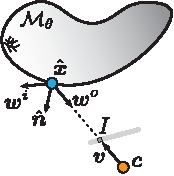
\includegraphics[width=0.25\textwidth]{notation.pdf}
  \end{center}\vspace{-20pt}
  \caption{Notations.}\label{fig:notation}
\end{wrapfigure}
%
with learnable parameters $\theta\in\Real^m$, a camera located at $\vc\in\Real^3$ and direction $\vv\in\gS$, where $\gS$ is the unit sphere, we would like to express the pixel color $I\in[0,1]$ (assume a single channel for now),  defined as the amount of light entering the camera $\vc$ in direction $\vv$, as a differentiable function of the surface parameters $\theta$. 
%
Of-course, aside from the geometry of the surface $\gM_\theta$, $I$ depends on material properties of the surface and scene lighting. 


Our goal is define a \emph{Universal Differentiable Rendered} (UDR), which is a neural network $R$ with parameters $(\theta,\gamma)\in\Real^{m+n}$ that satisfies the following: For arbitrary material and lighting conditions there exists $\gamma\in\Real^n$ so that $R(\vc,\vv;\theta,\gamma)$ approximates $I$ for different geometries $\gM_\theta$, camera location $\vc$ and direction $\vv$.   


\subsection{Notations and the rendering equation}
Let $\vhx=\vhx(\vc,\vv,\theta)$ denote the first intersection of the ray $\set{\vc+t\vv\vert t\geq 0}$ with the surface $\gM_\theta$, and $\vhn=\vhn(\vc,\vv,\theta)$ the normal to $\gM_\theta$ at $\vhx$. 
The pixel color $I$ equals the light reflected from $\gM_\theta$ at $\vhx$ in direction $-\vv$ reaching $\vc$. It is calculated by two functions: The bidirectional reflectance distribution function (BRDF) describing the reflectance and color properties of the surface, and the light emitted in the scene (\ie, light sources).

The BRDF function $f^r(\vx,\vn,\vw^o,\vw^i)$ describes the proportion of reflected radiance (\ie, flux of light) at some wave-length (\ie, color) leaving the surface point $\vx\in\Real^3$ with normal $\vn\in\gS$ at direction $\vw^o\in\gS$ with respect to the incoming radiance from direction $\vw^i\in\gS$. We let the BRDF depend also on the normal $\vn$ to the surface at a point; BRDFs are usually defined with respect to the normal, although, usually, this dependence is not made explicit due to the standard assumption that the geometry is fixed, which isn't the case here. 
%
The light sources in the scene are described by a function $L^e(\vx,\vw^o)$ measuring the emitted radiance of light at some wave-length at point $\vx\in\Real^3$ in direction $\vw^o\in\gS$. 

The amount of light reaching $\vc$ in direction $\vv$ equals the amount of light reflected from $\vhx$ in direction $\vw^o=-\vv$ and is described by the so-called rendering equation \cite{kajiya1986rendering,immel1986radiosity}:
\begin{equation}\label{e:render}
    L(\vhx,\vw^o) = L^e(\vhx,\vw^o)+\int_{\Omega} f^r(\vhx,\vhn,\vw^i,\vw^o) L^i(\vhx,\vw^i)(\vhn \cdot \vw^i)\ d\vw^i 
\end{equation}
where $L^i(\vhx,\vw^i)$ encodes the incoming radiance at $\vhx$ in direction $\vw^i\in\gS$, and the term $\vhn\cdot\vw^i$ compensates for the fact that the light does not hit the surface orthogonally; $\Omega$ is the half sphere defined by $\vhn$; the rendering equation holds for every light wave-length; as described later we will use it for the red, green and blue (RGB) wave-lengths. 

\subsection{Restricted BRDF and lighting model}
We restrict our material and lighting settings to those represented by a volumetric (continuous) BRDF function $f^r:\Real^3\times \gS \times \gS \times \gS\too \Real$ and light radiance functions $L^e,L^i:\Real^3\times \gS \too \Real$. We denote the collection of such continuous functions by $\gP=\set{(f^r,L^e,L^i)}$. This model includes many common materials and lighting conditions such as the popular Phong model \cite{foley1996computer}:
\begin{equation}\label{e:phong}
    L(\vhx,\vw^o)=k_d O_d I_a + k_d O_d I_d\parr{\vhn\cdot \frac{\vell-\vhx}{\norm{\vell-\vhx}}}_+ + k_s O_s I_d \parr{\vhr\cdot \frac{\vell-\vhx}{\norm{\vell-\vhx}}}_+^{n_s},
\end{equation}
where $(a)_+=\max\set{a,0}$; $k_d,k_s$ are the diffuse and specular coefficients, $I_a,I_d$ are the ambient and point light source colors, $O_d,O_s$ are the diffuse and specular colors of the surface, $\vell\in\Real^3$ is the location of a point light source, $\vhr=-(\mI-2\vhn\vhn^T)\vw^o$ the reflection of the viewing direction $\vw^o=-\vv$ with respect to the normal $\vhn$, and $n_s$ is the specular exponent. 
%Note that the Phong model can be written as $L(\vx,\vw^o)=R(\vx,\vn,\vw^o)$

The family $\gP$, however, does not include all possible lighting conditions, \eg, it excludes self-shadows and second order (or higher)  light reflections as $L^i$ is independent of the geometry $\gM_\theta$. 

\subsection{Universal Differentiable Renderer}
\label{ss:udr}
Our goal is to learn geometry $\gM_\theta$ in a scene via rendered images of this geometry under a wide range of materials and lighting conditions. We would like to be able to express these possible appearances of $\gM_\theta$ with arbitrary material/lighting models in $\gP$. For that end we define:
%
\begin{definition}
Given a parametric surface family $\gM_\theta$, $\theta\in\Real^m$, a \emph{Universal Differentiable Renderer} (UDR) for $\gM_\theta$ is a  function $$R(\vc,\vv;\theta,\gamma)$$ differentiable in $\theta,\gamma$, where $\theta\in\Real^m$, $\gamma\in\Real^n$, $\vc\in\Real^3$, and $\vv\in\gS$, such that for arbitrary material/lighting $(f^r,L^i,L^e)\in \gP$ there exists $\gamma\in\Real^n$ so that $R(\vc,\vv;\theta,\gamma)$ is an arbitrary good approximation of the light amount enters camera $\vc\in\Real^3$ in direction $\vv\in\gS$, \ie, $L(\vhx,-\vv)$, for all $\theta,\vc,\vv$ in some compact domain. 
\end{definition}
Given a UDR $R$, we can write down a loss consisting of terms of the form 
\begin{equation}\label{e:loss}
    \loss_{\scriptscriptstyle \mathrm{R}}(\vc,\vv,\theta,\gamma)= \abs{R(\vc,\vv;\theta,\gamma) - I}.
\end{equation}
The fact that $R$ is a UDR will guarantee that we could match the appearance of geometry $\gM_\theta$ to a wide range of materials and lighting conditions.  Furthermore, the requirement that $R$ can approximate the rendered light function for arbitrary camera, direction and geometry will facilitate separation of geometry and material/lighting in the learning process. 


We will prove the following is a UDR for geometry $\gM_\theta$:
\begin{equation}\label{e:udr}
    R(\vc,\vv;\theta,\gamma) = M(\vhx,\vhn,\vv;\gamma),
\end{equation}
where $M$ is an MLP with parameters $\gamma\in\Real^n$, and $\vhx=\vhx(\vc,\vv,\theta)$, $\vhn=\vhn(\vc,\vv,\theta)$, as defined above. 


%
\begin{theorem}\label{thm:udr}
The renderer in \eqref{e:udr} is a UDR.
\end{theorem}
\begin{proof}
Let $\gM_\theta$ be a parametric family of surfaces. Pick an arbitrary material/lighting $(f^r,L^e,L^i)\in \gP$ . We need to show there is an MLP $M$ so that \eqref{e:udr} is an arbitrary good approximation of $L(\vhx,-\vv)$. \Eqref{e:render} implies that there exists a continuous function $F$ so that $L(\vhx,-\vv)=F(\vhx,\vhn,\vv)$ for all $\theta,\vc,\vv$.  Assuming $(\vhx,\vhn,\vv)$ are contained in some compact set $\gK$, we can approximate (arbitrarily well) $F$ over $\gK$ with an MLP $M$ using the universality theorems of MLPs, see \cite{hornik1989multilayer} and \cite{hornik1990universal} for approximation including derivatives. \qed
\end{proof}


\begin{figure}[t]
    \centering
    \begingroup
\setlength{\tabcolsep}{15pt} % Default value: 6pt
\renewcommand{\arraystretch}{1.5} % Default value: 1
    \begin{tabular}{c|c|c}
%\centering
    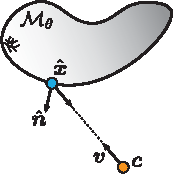
\includegraphics[width=0.2\columnwidth]{not_udr_a.pdf}&  
    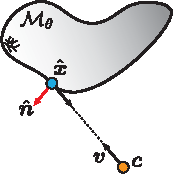
\includegraphics[width=0.2\columnwidth]{not_udr_b.pdf}&    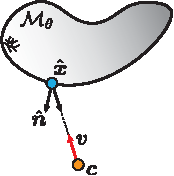
\includegraphics[width=0.2\columnwidth]{not_udr_c.pdf}\\
     (a) reference scene & (b) change in $\vhn$ & (c) change in $\vc$ and $\vv$  
\end{tabular}
\endgroup
    \caption{Differentiable renderers $R$ without $\vhn$ and/or $\vv$ are not universal; changing the surface normal (b) and/or the viewing direction (c) will produce different amount of light arriving the camera $\vc$ at direction $\vv$ and cannot be captured by $R$.}
    \label{fig:udr_no}
\end{figure}


An important question is: Are $\vhn,\vv$ necessary in \eqref{e:udr} in order to achieve a UDR? Previous works, \eg, \cite{niemeyer2019differentiable}, have considered rendering functions of the form 
\begin{equation}\label{e:udr_no_n_no_v}
    R(\theta,\vc,\vv;\gamma)=M(\vhx;\gamma).
\end{equation}
We will next prove this model is not a universal renderer. We will in fact show that removing $\vhn$ and/or $\vv$ from \eqref{e:udr} will result in a non-universal renderer. Assume $\gM_\theta$ is expressive enough to change the normal direction $\vhn$ arbitrarily at a point $\vhx$; for example, even a linear classifier $f(\vx;\va,b)=\va^T \vx+b$ would do. Let $M(\vhx;\gamma)$ be a UDR for $\gM_\theta$. Choose the Phong model (\eqref{e:phong}) and let $R(\theta,\vc,\vv;\gamma)=M(\vhx,\vv;\gamma)$ (\ie, remove the normal component from the renderer) be the light amount arriving at $\vc$ in direction $\vv$ as approximated by the renderer. Consider the setting shown in Figure \ref{fig:udr_no} (a) and (b): In both cases $M(\vhx,\vv;\gamma)$ yields the same value although changing the normal direction at $\vhx$ will produce, under the Phong model, a different light amount at $\vc$. 

Similarly, consider a renderer with the viewing direction ($\vv$) removed, \ie, $M(\vhx,\vhn;\gamma)$, and Figure \ref{fig:udr_no} (a) and (c): In both cases $M(\vhx,\vhn;\gamma)$ produces the same value although, under the Phong model, the reflected light can change when the point of view changes. That is, we can choose light position $\vell$ in \eqref{e:phong} so that different amount of light reaches $\vc$ at direction $\vv$. 

%\yl{discuss the fact that latent cannot help?}


\subsection{Implementation of the UDR}
To implement the UDR in \eqref{e:udr} we first represent the geometry $\gM_\theta$ as in \eqref{e:gM} using an MLP $f:\Real^m\too\Real$. We enforce $f$ to be approximately signed distance function with Implicit Geometric Regularization (IGR) \cite{gropp2020implicit}, \ie, incorporating the Eikonal regularization term 
\begin{equation}\label{e:eikonal}
\loss_{\scriptscriptstyle\mathrm{E}}(\theta) = \E_{\vx} \big(\norm{\nabla_\vx f(\vx;\theta)}-1\big)^2
\end{equation}
where $\vx$ is distributed uniformly in a bounding box of the scene. 

Next, we need to have $\vhx(\vc,\vv,\theta)$, and $\vhn(\vc,\vv,\theta)$ both differentiable in $\theta$. $\vhx$ requires representing the location of a point on $\gM_\theta$ using the parameters $\theta$ of $f$. This was recently done in \cite{atzmon2019controlling,niemeyer2019differentiable}; we employ the sample network idea from \cite{atzmon2019controlling}. That is, as we show in the supplementary material, let $\theta_0$ denote the current parameter, a first-order approximation to $\vhx$ is
\begin{equation}\label{e:vhx}
    \vhx(\vc,\vv,\theta) = \vhx_0 - \vu f(\vhx_0;\theta)
\end{equation}
where $\vhx_0=\vhx(\vc,\vv,\theta_0)$, and $\vu=\frac{\vv}{\nabla_\vx f(\vhx_0;\theta_0) \cdot \vv}$ are constant vectors. The benefit in \eqref{e:vhx} is that it can be implemented by adding a single linear layer to the MLP $f$; 
%
$\vhx_0$ is computed using the sphere tracing algorithm similar to  \cite{liu2019dist}.
%
The term $\vhn(\vc,\vv,\theta)$ is the normal to $\gM_\theta$ at point $\vhx$. Since $f$ is approximately a sign distance function we set 
\begin{equation}\label{e:vhn}
\vhn(\vc,\vv,\theta)=\nabla_\vx f( \vhx(\vc,\vv,\theta) ; \theta ).
\end{equation}
The term $\nabla_\vx f(\vx ; \theta)$ in equations \ref{e:eikonal} and \ref{e:vhn} is implemented using a version of automatic differentiation of the MLP $f$, by building a networks that computes $(f(\vx;\theta),\nabla_\vx f(\vx;\theta))$ in the forward-pass, as suggested in \cite{gropp2020implicit}. Lastly, we incorporate equations \ref{e:vhx}-\ref{e:vhn} with an MLP $M$ to get our UDR, \eqref{e:udr}; $M$ outputs 3 RGB values. 

\subsection{Loss function for multi-view reconstruction}
Let $I_j\in [0,1]^3$, $\alpha_j\in[0,1]$ be the RGB values and the opacity value corresponding to a pixel in an image taken with camera $\vc_j\in\Real^3$ and direction $\vv_j\in\gS$ where $j\in J$, see Figure \ref{fig:notation}. That is, $J$ indexes all the pixels in a collection of images. 

Let $f(\vx;\theta)$ be an MLP where $\gM_\theta$ represents the reconstructed surface with current parameter $\theta=\theta_0$. For each $j\in J$ we perform sphere-tracing \cite{jiang2019sdfdiff} to compute $\vhx_j=\vhx_j(\vc_j,\vv_j,\theta_0)$. Let $J^{\scriptscriptstyle \mathrm{in}}\subset J$ be the subset of indices where $\vhx_j$ was found; $J\setminus J^{\scriptscriptstyle \mathrm{in}}$ are therefore the indices of pixels where the ray $\set{\vc_j+t\vv_j\vert t\geq 0}$ did not intersect $\gM_\theta$. 
Then our loss is
\begin{align}\label{e:loss_full}
    \loss(\theta,\gamma)    = &    \sum_{j\in J^{\scriptscriptstyle \mathrm{in}}} \Big(\alpha_j\loss_{\scriptscriptstyle\mathrm{R}}(\vc_j,\vv_j,\theta,\gamma) - \tau(1-\alpha_j)f({\vy}_j;\theta)  \Big ) \\ \nonumber & + \tau\sum_{j\in J\setminus J^{\scriptscriptstyle \mathrm{in}}} \alpha_j f({\vz}_j;\theta) +\lambda\,\loss_{\scriptscriptstyle \mathrm{E}}(\theta),
\end{align}
where $\lambda,\tau>0$ are constant parameters, $\loss_{\scriptscriptstyle\mathrm{E}}$ is defined in \eqref{e:eikonal}, $\loss_{\scriptscriptstyle \mathrm{R}}$ is defined in \eqref{e:loss},  $\vy_j$ is the point along the ray $\set{\vhx_j+t\vv\vert t\geq 0}$ that minimizes $f(\cdot\, ;\theta)$, and $\vz_j$ is the point along the ray $\set{\vc_j+t\vv\vert t\geq 0}$ that minimizes $f(\cdot\,;\theta)$; both $\vy_j,\vz_j$ are independent of $\theta$. The two terms including $\vy_j,\vz_j$ are treating cases where the opacity coefficient $\alpha_j,(1-\alpha_j)$ is in conflict with the existent/nonexistent intersection of the ray $\set{\vc+t\vv\vert t\geq 0}$ and $\gM_\theta$. 

%Lastly, we initialize the parameters $\theta$ of $f$ using the geometric initialization \cite{atzmon2019sal}.
%\yl{matan initialiation}


\begin{figure}[t]
    \centering
    \begingroup
\setlength{\tabcolsep}{10pt} % Default value: 6pt
    \begin{tabular}{ccc}
         \includegraphics[width=0.25\columnwidth]{color/udr/sphere_udr.png} &
         \includegraphics[width=0.25\columnwidth]{color/udr_minus/sphere_udr_minus.png} &   \includegraphics[width=0.25\columnwidth]{color/dvr/sphere_dvr.png}  \\
          UDR & DRnoV & DVR 
    \end{tabular}
    \endgroup
    \caption{Shiny sphere test (Phong reflection model). The geometry $\gM_\theta$ reconstructed by the UDR, DVR, and DRnoV models.}
    \label{fig:sphere_geometry}
\end{figure}

\pagebreak
\section{Experiments}

We compared our UDR model, \eqref{e:udr}, to the Differentiable Volumetric Rendering (DVR) \cite{niemeyer2019differentiable}, namely $R(\vc,\vv;\theta,\gamma) = M(\vhx;\gamma)$, and to a model similar to UDR but without the view direction (DRnoV), $R(\vc,\vv;\theta,\gamma) = M(\vhx,\vhn;\gamma)$.

\paragraph{Implementation details.}
We represent the geometry $\gM_\theta$ using an MLP $f(\vx;\theta)$,  $f:\Real^3\times\Real^m\too\Real$, consisting of 8 layers with hidden dimension of size 512, and a single skip connection from the input to the middle layer as in \cite{park2019deepsdf}. We initialize the weights $\theta\in\Real^m$ using the geometric initialization from \cite{atzmon2019sal}; this provides a close to sign distance function already at initialization. For the implementation of the UDR we use also an MLP, $M(\vhx,\vhn,\vv;\gamma)$, $M:\Real^3\times\Real^3\times \Real^3\times \Real^n \too \Real^3$, consisting of of 4 layers, with 512 hidden units. In our loss, \eqref{e:loss_full}, we set the constant parameters to be $\lambda=0.1$ and $\tau=5$.


\begin{figure}[t]
\centering
    \begin{tabular}{ccccc}
         \includegraphics[width=0.2\columnwidth]{color/dvr/eval_10000_4.png} &  
         \includegraphics[width=0.2\columnwidth]{color/dvr/eval_10000_1.png} &
         \includegraphics[width=0.2\columnwidth]{color/dvr/eval_10000_2.png} &
         \includegraphics[width=0.2\columnwidth]{color/dvr/eval_10000_3.png} &
         \includegraphics[width=0.2\columnwidth]{color/dvr/eval_10000_9.png} \vspace{-10pt} \\ 
         & & {DVR} & & \\
         %%%%%%%%%%%%%%%%%%%%%%%%%%%%%%%%%
         \includegraphics[width=0.2\columnwidth]{color/udr_minus/eval_10000_3.png} &  
         \includegraphics[width=0.2\columnwidth]{color/udr_minus/eval_10000_6.png} &
         \includegraphics[width=0.2\columnwidth]{color/udr_minus/eval_10000_8.png} &
         \includegraphics[width=0.2\columnwidth]{color/udr_minus/eval_10000_0.png} &
         \includegraphics[width=0.2\columnwidth]{color/udr_minus/eval_10000_7.png} \vspace{-10pt} \\ 
         & & {DRnoV} & & \\
         %%%%%%%%%%%%%%%%%%%%%%%%%%%%%%%%%
         \includegraphics[width=0.2\columnwidth]{color/udr/eval_10000_1.png} &  
         \includegraphics[width=0.2\columnwidth]{color/udr/eval_10000_9.png} &
         \includegraphics[width=0.2\columnwidth]{color/udr/eval_10000_0.png} &
         \includegraphics[width=0.2\columnwidth]{color/udr/eval_10000_4.png} &
         \includegraphics[width=0.2\columnwidth]{color/udr/eval_10000_3.png} \vspace{-10pt} \\ 
         & & {UDR} & & \\
         %%%%%%%%%%%%%%%%%%%%%%%%%%%%%%%%%
         \includegraphics[width=0.2\columnwidth]{color/gt/eval_10000_4.png} &  
         \includegraphics[width=0.2\columnwidth]{color/gt/eval_10000_1.png} &
         \includegraphics[width=0.2\columnwidth]{color/gt/eval_10000_2.png} &
         \includegraphics[width=0.2\columnwidth]{color/gt/eval_10000_3.png} &
         \includegraphics[width=0.2\columnwidth]{color/gt/eval_10000_9.png} \vspace{-10pt} \\ 
         & & {Ground Truth} & & \\
         %%%%%%%%%%%%%%%%%%%%%%%%%%%%%%%%%
    \end{tabular}
    \caption{Shiny sphere test (Phong reflection model). Columns represent renderings from unseen camera locations and directions. Each row is produced by (from top to bottom): DVR, DRnoV, UDR and ground truth. Note that as predicted from the theory, only UDR is able to render faithful images of the shiny sphere.}
    \label{fig:sphere_test_images}
\end{figure}

\subsection{Shiny sphere test}
We evaluate the different differentiable renderers with a simple sphere geometry with a strong specularity generated with a Phong reflection model (\eqref{e:phong}). We have generated 50 train images of size $256\times 256$ pixels from random camera locations pointing toward the sphere's center and trained geometry $\gM_\theta$ and the different renderers $R$ via minimization of the loss in \eqref{e:loss_full}. Figure \ref{fig:sphere_geometry} depicts the reconstructed geometries $\gM_\theta$ with the different renderers: UDR, DrnoV, and DVR; Figure \ref{fig:sphere_test_images} depicts images from unseen camera locations and directions created using the trained geometry and different renderers. As can be observed, and as suggested by the theory in Section \ref{ss:udr}, UDR is able to separate well geometry and reflectance, reproducing the sphere shape and near perfect renderings; the baselines, on the other hand, tend to confuse lighting and geometry and do not reconstruct the sphere shape or the lighting properties of the scene. 


 


\subsection{3D reconstruction with multiview supervision}\label{exp_recon}
In this experiment we tested reconstruction of 3D models using the image dataset of Choy et al.\cite{choy20163d}. This dataset contains 13 model categories from the ShapeNet dataset \cite{shapenet2015}, where each model has 24 rendered images of size $137\times 137$ with known camera parameters and opacity channel. We have taken the first 10 models in each category and for each model we tested each of the renderers mentioned above. That is, for each model, we extracted the per-pixel information $(I_j,\alpha_j,\vc_j,\vv_j)$, $j\in J$, from the 24 images, and optimized the loss in \eqref{e:loss_full} to find the geometry $\gM_\theta$ and renderer network $M$ for each model.


%\pagebreak

\paragraph{Evaluation.}
We evaluate the accuracy of the 3D surface reconstruction ($\gM_\theta$) and rendered images of the different renderers ($R$) from the input directions. The 3D reconstruction accuracy is measured with the standard Chamfer-$L_2$ distance: $$
d_{\text{C}}\left(\gX_{1},\gX_{2} \right) = d\left(\gX_{1},\gX_{2} \right) + d\left(\gX_{2},\gX_{1} \right),
$$ where
$$ d\left(\gX_{1},\gX_{2} \right) = \frac{1}{\abs{\gX_1}}\sum\limits_{\vx_{1}\in\gX_{1}}\min\limits_{\vx_2\in \gX_{2}}\norm{\vx_1-\vx_2},$$ and $\norm{\cdot}$ is the 2-norm.
%
We also measure the PSNR of our renderings compared to the input 24 images. Table \ref{tab:multiview_reconstruction} log the results; Figures \ref{fig:recon1}, \ref{fig:recon2} depict the ground truth models, reconstructed 3D geometry with DVR and UDR, examples of the input images, and rendered (higher-res) images from unseen directions using the trained renderers. Note that our method compares favorably to the baseline and provide more accurate 3D reconstructions as well as renderings from unseen directions.    

\begin{wrapfigure}[12]{r}{0.5\columnwidth}
     \centering \vspace{-30pt}
     \includegraphics[width=0.4\columnwidth]{failure.png}\vspace{-10pt}
     \caption{Failure cases of UDR. From left to right: ground truth, UDR reconstruction, UDR rendering, and example input images.}
     \label{fig:fail}
\end{wrapfigure}


\subsection{Method limitations}
Figure \ref{fig:fail} shows some typical failure cases, illustrating the difficulties of our method with 3D reconstructions of thin objects, and generalization to unseen parts. The generalization to unseen parts could be potentially resolved by learning shape space, collecting information of the shape from different by similar shapes. Lastly, note the low resolution of the input images, a fact which can explain some of artifacts in out results.


\begin{table}[t]
    \hspace{-20pt}
    \setlength\tabcolsep{8pt} % default value: 6pt
    \begin{tabular}{c}
        \begin{adjustbox}{max width=\textwidth}
        \renewcommand{\arraystretch}{1.1}
        \begin{tabular}[t]{l||ccc|ccc}
            \toprule
             &
            \multicolumn{3}{c|}{\textbf{Chamfer-$L_2$}} & 
            \multicolumn{3}{c}{\textbf{PSNR}} \\
        % \midrule
        Category & DVR \cite{niemeyer2019differentiable} & DRnoV & UDR &  DVR \cite{niemeyer2019differentiable} & DRnoV & UDR \\
         \midrule 
        Airplane & $0.72\pm0.71$ & $3.28\pm3.47$ & $\mathbf{0.55}\pm0.16$ &
        $24.89\pm2.13$ & $23.88\pm3.54$ & $\mathbf{25.47}\pm2.57$ \\
        Bench & $3.45\pm2.09$ & $3.64\pm3.24$ & $\mathbf{1.8}\pm1.61$ &
        $19.89\pm4.39$ & $21.26\pm4.93$ & $\mathbf{22.61}\pm3.58$ \\
        Cabinet &$1.63\pm1.19$ & $1.63\pm1.07$ & $\mathbf{1.25}\pm1.05$ &
        $23.9\pm3.88$ & $24.11\pm4.19$ & $\mathbf{25.83}\pm3.89$ \\
        Car & $\mathbf{1.15}\pm0.34$ & $1.36\pm0.77$ & $1.53\pm0.83$ & 
        $19.8\pm1.58$ & $\mathbf{21.15}\pm1.91$ & $21.14\pm1.67$ \\
        Chair & $4.63\pm5.62$ & $3.06\pm3.74$ & $\mathbf{1.95}\pm3.09$ &
        $20.21\pm3.98$ & $20.94\pm4.14$ & $\mathbf{22.01}\pm3.97$ \\
        Display & $0.95\pm0.68$ & $1.21\pm1.58$ &$\mathbf{0.67}\pm0.26$ & 
        $22.59\pm4.64$ & $23.76\pm3.91$ & $\mathbf{25.22}\pm3.86$ \\
        Lamp & $3.04\pm3.0$ & $2.3\pm1.66$ & $\mathbf{1.31}\pm1.04$ &
        $22.29\pm3.54$ & $22.13\pm3.46$ & $\mathbf{23.62}\pm3.17$ \\
        Speaker & $\mathbf{1.79}\pm1.04$ & $1.95\pm1.69$ & $2.49\pm2.62$ &
        $\mathbf{23.03}\pm3.15$ & $23.31\pm3.63$ & $23.69\pm4.79$ \\
        Rifle & $0.42\pm0.3$ & $\mathbf{0.35}\pm0.29$ & $0.73\pm0.64$ & 
        $23.29\pm2.58$ & $\mathbf{23.63}\pm2.81$ & $23.24\pm2.81$ \\
        Sofa & $2.02\pm1.6$ & $3.07\pm2.76$ & $\mathbf{1.42}\pm0.8$ &
        $23.03\pm2.68$ & $23.0\pm3.05$ & $\mathbf{25.21}\pm3.14$ \\
        Table & $3.3\pm2.19$ & $3.27\pm1.93$ & $\mathbf{1.06}\pm1.06$ & 
        $20.43\pm3.7$ & $21.59\pm4.91$ & $\mathbf{23.97}\pm3.59$ \\
        Telephone & $0.7\pm1.02$ & $\mathbf{0.34}\pm0.28$ & $0.4\pm0.43$ &
        $23.34\pm4.34$ & $23.76\pm3.61$ & $\mathbf{24.37}\pm3.0$ \\
        Vessel & $1.72\pm2.05$ & $1.33\pm1.59$ & $\mathbf{0.96}\pm0.8$ &
        $24.82\pm2.6$ & $25.62\pm2.79$ & $\mathbf{26.45}\pm2.63$ \\
        \bottomrule
              \end{tabular} 
        \end{adjustbox}
      
    \end{tabular}
    \vspace{3pt}
    \caption{Multiview 3D reconstruction, quantitative results. We report $L_2$ Chamfer distance (multiplied by $10^3$, mean $\pm$ std) between the reconstructed 3D surface and the ground truth; and PSNR (in dB, mean $\pm$ std) of the rendered images using the trained renderers and input images. } %\vspace{-15pt}
    \label{tab:multiview_reconstruction}
\end{table}
  
  
 \section{Conclusions}
 We have introduced the Universal Differentiable Renderer (UDR) that, as far as we are aware, is the first neural network architecture that can provably approximate a wide range of appearances (material/lighting) of 3D geometries represented as zero level sets of neural networks. 
 A current limitation of the method seems to be the rather heavy computational complexity of the training, requires computing sphere tracings of many pixels in each iteration of the algorithm. Incorporating different acceleration techniques and/or importance sampling could alleviate the situation and we mark it as future work. 
 Another future work direction is to incorporate the UDR in other computer vision and learning applications such as 3D model generation, structure from motion, and learning 3D models from images without known camera properties. 
 
 
 
\begin{figure}[t]
    \centering
    \includegraphics[width=\textwidth]{lior_1.jpg}
    \caption{Multiview 3D reconstruction, qualitative results (A). We show (left to right): ground truth geometry, DVR reconstruction, UDR reconstruction, examples of input images, and 2 renderings from unseen directions.}
    \label{fig:recon1}
\end{figure}
 
\begin{figure}[t]
    \centering
    \includegraphics[width=\textwidth]{lior2.jpg}
    \caption{Multiview 3D reconstruction, qualitative results (B). We show (left to right): ground truth geometry, DVR reconstruction, UDR reconstruction, examples of input images, and 2 renderings from unseen directions. }
    \label{fig:recon2}
\end{figure}



\clearpage

 
% ---- Bibliography ----
%
% BibTeX users should specify bibliography style 'splncs04'.
% References will then be sorted and formatted in the correct style.
%



\bibliographystyle{splncs04}
\bibliography{rendering_arxiv}

\clearpage

\section{Supplementary Material}
\subsection{Directional Sample Network}
Let the point $\vx$ be the intersection of $\gM_\theta$ and the ray $\set{\vc+t\vv \vert t\geq 0}$, where $\vc\in\Real^3$ is the camera center and $\vv\in\gS$ is the viewing direction. That is 
\begin{equation}\label{e:intersection}
    \vx(\vc,\vv,\theta) = \gM_\theta \cap \set{\vc+t\vv \ \vert \ t\geq 0}.
\end{equation}
We want to produce a first order approximation $\vhx$ to $\vx$ at $\theta=\theta_0\in\Real^m$, that is a neural network $\vhx(\vc,\vv,\theta)$ so that 
\begin{equation}\label{e:dsn_1}
  \vhx(\vc,\vv,\theta_0)=\vhx_0,  
\end{equation}
where $\vhx_0=\vx(\vc,\vv,\theta_0)$, and
\begin{equation}\label{e:dsn_2}
  \nabla_\theta \vhx(\vc,\vv,\theta_0)= \nabla_\theta \vx(\vc,\vv,\theta_0).  
\end{equation}
We will use the sample network from \cite{atzmon2019controlling}.
In particular, we prove that \eqref{e:vhx} in the main paper, namely the network constructed by adding a single linear layer to the MLP $f$,
\begin{equation}\label{e:vhx_app}
    \vhx(\vc,\vv,\theta) = \vhx_0 - \vu f(\vhx_0;\theta)
\end{equation}
$\vu=\frac{\vv}{\nabla_\vx f(\vhx_0;\theta_0) \cdot \vv}$, satisfies these conditions. 

First, \eqref{e:dsn_1} holds since $f(\vhx_0;\theta_0)=0$. Second, to show \eqref{e:dsn_2} we note that $f(\vx;\theta)\equiv 0$. 
Using the chain rule and setting $\theta=\theta_0$ we get:
\begin{equation}\label{e:cond}
  \frac{\partial f(\vhx_0;\theta_0)}{\partial \theta} +  \nabla_\vx f(\vhx_0;\theta_0)^T\frac{\partial \vx (\vc,\vv,\theta_0)}{\partial \theta}=0.    
\end{equation}
Next, by \eqref{e:intersection}, $\frac{\partial \vx(\vc,\vv,\theta_0)}{\partial \theta} = \vv\vw^T$, for some $\vw\in\Real^m$. Plugging this back in \eqref{e:cond} and solving for $\vw$ yields 
$$\vw^T=-\frac{1}{\nabla_\vx f(\vhx_0;\theta_0) \cdot  \vv}  \frac{\partial f(\vhx_0;\theta_0)}{\partial \theta}.$$
Finally, notice that $\frac{\partial \vhx (\vc,\vv,\theta_0)}{\partial \theta}=\vv\vw^T$. 

\subsubsection*{Relation to \cite{niemeyer2019differentiable}.}
Implicit differentiation, as in \eqref{e:cond}, has been exploited recently also in \cite{niemeyer2019differentiable}. However, our implementation differs in deriving the sample network in \eqref{e:vhx_app}; the benefit in the sample network is that it is easily implemented by adding a fixed linear layer to the MLP $f$ for every sample point $\vhx_0$, see \cite{atzmon2019controlling} for more details. As the UDR model (see \eqref{e:udr}) additionally requires surface normals, our use of the sample network allows us to achieve a differentiable normal representation, $\vhn(\vc,\vv,\theta)=\nabla_\vx f( \vhx(\vc,\vv,\theta) ; \theta )$, as well. Note that $\nabla_\vx f$ represents the normal direction of the level sets of a signed distance function (SDF); one could explicitly normalize $\nabla_\vx f / \norm{\nabla_\vx f}$ to get the precise normal, even for approximate or non-SDF; however, we worked with $\vhn$ as detailed. 

\subsection{Implementation Details}
\subsubsection{Sphere tracing.}
Given a camera position $\vc$ and a direction $\vv\in\gS$ that together characterize some pixel location, 
we performed sphere tracing along the ray $\set{\vc+t\vv\ \vert \ t\geq 0}$ to find the corresponding surface sample $\vhx_0$ from $\gM_{\theta}$. As $\gM_\theta$ is defined by an approximate sign distance field $f$ we opted for sphere tracing algorithm \cite{hart1996sphere}. In Algorithm \ref{a:sphere} we describe the details of our implementation for the sphere tracing algorithm.\\\\
\begin{algorithm}[H]\label{a:sphere}
 \caption{Sphere tracing}
\SetAlgoLined
 \KwData{Initial point $\vp_0$, ray direction $\vv$}
 \KwResult{The intersection $\vx=\gM_{\theta_0}\cap\set{\vp_0+t\vv\vert t\geq 0}$}
 $\vx = \vp_0$\;
 \While{$f\left(\vx;\theta_0\right) > \epsilon \text{ and } \norm{\vx}_2 < r $}{
  $d = f\left(\vx;\theta_0\right)$;\\
  \If{$f\left(\vx + d\vv ;\theta_0\right) < 0$}{
   $d = \alpha \cdot d$
   }
   $\vx = \vx + d \vv$\;
 }
\end{algorithm}
\vspace{10pt}
The algorithm uses the following parameters: $\epsilon>0$ is the convergence threshold, and $r>0$ is the radius of the bounding sphere of the object (we assume the objected is centered at the origin). For all of our experiments we set $\epsilon = 1\mathrm{e}{-5}$, and $r = 1$. Moreover, we set $\alpha = 0.5$, used to make conservative distance estimations in case $f$ is not a perfect signed distance function.
%
$\vp_0$ is the initialized point for the algorithm and usually defined as the camera center, $\vp_0 = \vc$. In order to accelerate the process we took $\vp_0$ as the first intersection point of the ray $\set{\vc+t\vv\vert t\geq 0}$ and the bounding sphere $\set{\vx\, \vert \norm{\vx}_2\leq r}$, as done in \cite{liu2019dist}.
We parallelized this process on the GPU for multiple views and directions $\left\{(\vc_j,\vv_j)\right\}$. 

\subsubsection{Training Details.}
We trained using the \textsc{Adam} optimizer \cite{kingma2014adam} with $1\mathrm{e}{-4}$ as our learning rate, setting for each step the number of views to $24$ and the number of sampled pixels to $1024$. All models were trained for $10$K epochs. Training was done on a single Nvidia V-100 GPU, using \textsc{pytorch} deep learning framework \cite{paszke2017automatic}.\\
Regarding the loss in \eqref{e:loss_full}, we find $\vy_j$ and $\vz_j$ by randomly sampling the ray $\set{\vhx_j+t\vv\vert t\geq 0}$ and $\set{\vc_j+t\vv\vert t\geq 0}$ accordingly, and took the points that minimize $f(\cdot\, ;\theta)$.

\subsection{Additional Results}
Figure \ref{fig:recon3} depicts additional results from the multiview 3D reconstruction experiment described in section \ref{exp_recon}.
\begin{figure}[t]
    \centering
    \includegraphics[width=\textwidth]{lior_3.jpg}
    \caption{Multiview 3D reconstruction, qualitative results (C). We show (left to right): ground truth geometry, DVR reconstruction, UDR reconstruction, examples of input images, and 2 renderings from unseen directions.}
    \label{fig:recon3}
\end{figure}

\end{document}
